\chapter{Introduction}

Welcome to the early days of home computing.

Let's make a journey to the 1980s. During that decade, the computing industry experienced a big revolution. The lessons learned during the 70s pointed at a future where computers domain everything. A future in which computers will be everywhere: in the businesses, in the offices, in the industries... and of course, in our homes.

During these days, many companies produced what was called home computers. It is the age of the Spectrum ZX, the Commodore 64, the Amstrad CPC, and of course the big family of MSX computers. Microcomputers with short capabilities and resources found their place in our homes when we were just kids. We learned to play video-games with these early computers. We learned to code with them. We learned their potential. Their power to transform the World. And we learned all that was just the beginning.

Again, welcome to the early days of home computing. Welcome to Artemisa.

\section{What is Artemisa}

Artemisa is an 8-bit computer system that implements the MSX-1 specification. There were many hardware vendors who produced MSX computers in the 80s. Sony, Canon, Casio, Sharp, Spectravideo, Panasonic, Philips, ... Artemisa is just another member of this big family, with some particularities.

One of these particularities is that the design of the Artemisa started in 2018. That is 35 years after the initial design of the first MSX computers. But actually this is  not new. In 2006, ESE Artists’ Factory designed the 1chipMSX. This is a FPGA-based computer system that implements the MSX-2 standard. In 2013, a Korean team of MSX enthusiasts known as Retroteam Neo created the Zemmix Neo as an evolution of the 1chipMSX design with inspiration from the classic Zemmix game console produced by Daewoo. Since then, many other teams along the globe had produced their own customizations of Zemmix Neo. Also, in 2020 a group of Spanish makers released the MSXVR. This is an enhanced MSX emulated by a Raspberry Pi with the physical appearance of a classic 8-bit computer.

So yes, Artemisa is just another member that joins the club of MSX computers designed in 21st century. But here comes another particularity. Artemisa is one of the few, along the Omega MSX, that do not use emulation techniques. Some other products as 1chipMSX or Zemmix Neo use FPGAs to emulate the whole MSX hardware. Some others as the MSXVR or the Zemmix Mini uses software emulation on top of an ARM-based computer running GNU/Linux. In contrast, Artemisa (and also Omega) use real integrated circuits and discrete logic. In other words, it is made using the same design techniques and materials used in the 80s, when the first MSX computers were also designed. For example, the heart of the Artemisa computer is a real Zilog Z80 microprocessor instead of a Z80 CPU reimplemented in an HDL language by reverse engineering and synthetized in a typical Altera Cyclone FPGA.

Please note this does not mean Artemisa is better (or worse) than its FPGA-based or software-based counterparts. It is likely that all the things you can do with Artemisa can also be done in any other MSX computer system, emulated or not. You will not observe any remarkable additional feature, more speed or more stability. All them are functional MSX computers you can enjoy.

\section{Why Artemisa?}

You might ask why you would need an Artemisa computer considering there are some other options out there. Good question!

One possible answer is that you might find Artemisa computer more authentic. Please note I am not saying it is actually more authentic. But just you might feel that. There are some users that specially appreciate the classic hardware. And they feel more comfortable using an MSX computer that uses the classic technologies, implemented with a real CPU, real VDP, real PSG, real memory, … A computer that is designed using the old-school techniques with bare metal. In contrast, some other users do not care. They do not have a different experience using an emulator than using a traditional computer. If you think you belong to the former group of users, you will enjoy Artemisa. If not, it is yet another MSX computer.

In the case of Artemisa Homebrew DIY series, there is another reason for choosing it. You will have the chance to learn how an MSX computer is designed from the top to the bottom. And I am not just saying that because you will have to assemble it. Thanks to this book, you will also have the chance to understand how every single chip works. You will have access to the schematic designs of every single circuit and an educational guide about their role and operation in the circuit. This is a complete lecture about the architecture and design of MSX computers. A book that will put in your hands the tools to understand how a microcomputer works from the top to the bottom. If you are interested in computer architectures beyond the theory, you will find Artemisa was made for your needs. 

In summary, there we have two good reasons to choose Artemisa: 
\begin{itemize}
	\item Because you feel the bare hardware is particularly sexy.
	\item Because you want to learn how an MSX computer works.
\end{itemize}

However, if you only want to have an MSX machine that just works and you are not particularly interested in any of these value propositions, probably other options are better. On one hand, a refurbished MSX or a new FPGA-based one are likely less expensive. On the other hand, some other homebrew designs such as the Omega are more powerful and MSX2-compliant, but they lack the extensive documentation to understand their design. The offer of Artemisa is educative. The goal is to make you learn computer architecture and design at the same time you build and assemble your own MSX computer using real hardware, chip by chip. 

The decision is up to you.

\section{About this document}

As stated above, this handbook compiles all the technical knowledge about the Artemisa Homebrew DIY Computer series. You will find it useful to assemble the parts of the DIY kit. But also, to understand how an MSX computer works in detail. From the smaller chip to its most complex circuit. 

\section{Intended audience}

If you have purchased an Artemisa Homebrew DIY Computer series, you are likely an electronic hobbyist or an MSX fan and you feel skilled enough to assemble a computer system by your own. This means soldering the components following the detailed instructions you will find in this book. 

The Artemisa model 101 is built using electronic components that use large through-hole packages. The integrated circuits used in the design are DIP (Dual Inline Package), with a pad separation of 2.54mm. Other components such as resistors and capacitors are also large. In general, small and space-saving packaging such as SMD (Surface Mount Device) are avoided. This not only resembles the design style of early 80s computers but also lowers the entrance barrier for those that do not trust their own soldering skills. The grade of difficulty of assembling an Artemisa computer model 101 is quite low. 

Thus, only a basic knowledge in soldering is required. If unsure, there are tons of guides in the Internet and hundreds of YouTube tutorials available online to learn how. Assembling this kind of electronic components is easy. Just forget your fears and enjoy the experience!

Also, if you want to take advantage of the educational opportunities of this book, some basic knowledge of computing and digital systems is required. The user is assumed to understand basic concepts such as bit, byte, memory address, bus, CPU, peripheral, logic gate, voltage level, etc. A degree in Computer Science is useful, but not necessary. However, you will make the most from this book if your knowledge is above the standard knowledge of a regular computer user.

\section{How to Read This Book}

There are some parts of the book that have a special meaning or must be read in some specific way. They are described in this section. 

\subsection{Theory of operation blocks}

These blocks will be represented as follows:

\begin{theory}{Theory of operation}
	Here goes a full detailed description of how a part of the circuit works. 	
\end{theory}

The theory of operation blocks will describe the theory behind a part of the system. A basic knowledge on computing and digital systems is required in order to fully understand these blocks. However, do not worry if you lack this knowledge or find it difficult to understand. This information is not essential to assemble the system. You can still build your Artemisa computer without fully understanding what these text blocks tell. This is just for educational purposes.

When some concept mentioned in the book is related to a theory of operation block, it will be indicated with a book-and-bulb symbol beside. For example, in \toref{this concept}.

\subsection{Warning blocks}

Some operations require special attention to things that, when unnoticed, could cause damage in the circuit. In these cases, a warning text block will indicate you have to pay special attention, like this one:

\begin{warning}[Warning message!]
	This is a warning message that requires your attention.
\end{warning}

\subsection{Schematic diagrams}

Along this document, the different parts of the circuit are explained using schematic diagrams. They are not difficult to understand. But if you are not familiarized at all with them, a brief introduction might be useful. 

Most of the elements you will find in a schematic diagram are shown in Figure \ref{fig:schematic-elements}.

\begin{figure}[h]
	\centering
	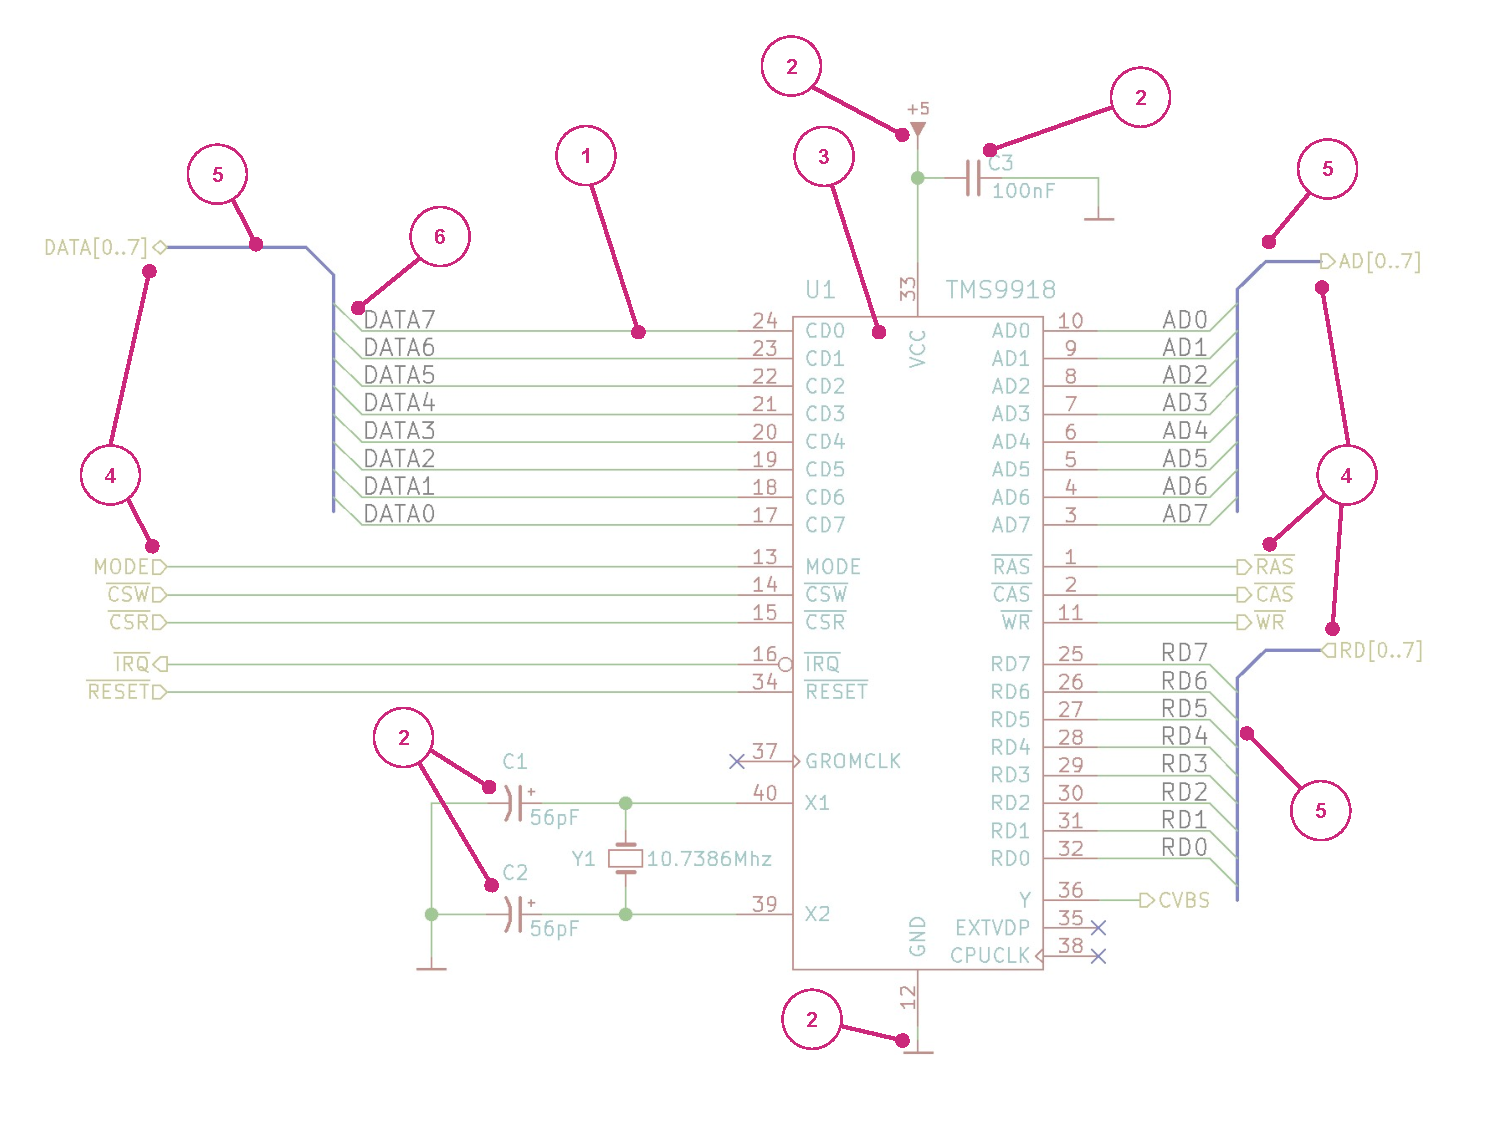
\includegraphics[width=\textwidth]{figures/schematic-elements}
	\caption{Elements of a schematic diagram}
	\label{fig:schematic-elements}
\end{figure}

\begin{enumerate}
	\item Wires. This is the most basic building block of a schematic diagram. It connects two points electrically. This means there will be a copper path between them in the circuit board that will let the current flow among these points.
	\item Basic components. Elements that have one or more pins where wires can be connected. These are power supply terminals, capacitors, resistors, oscillators, logic gates, etc. The different symbols used in this manual are described in Table \ref{table:schematic-symbols}.
	\item Integrated circuits. Components that contain a whole and complex circuit inside it. These are processors, memories, flip-flops, decoders, etc.
	\item Connections from/to other schematic diagrams. The pointing edge indicates the direction of the signal. If it has two pointed edges, it is bidirectional.
	\item Buses. Collections of parallel wires that transmit a multibit data.
	\item Wire connections from/to buses. A label indicates what is the wire that is obtained from the bus.
\end{enumerate}

\begin{table}[h!]
	\centering
	\begin{tabular}{ m{25mm}|l }
		\centering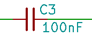
\includegraphics{icons/cap-cer}  & Ceramic capacitor      \\
		\centering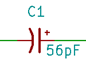
\includegraphics{icons/cap-elec} & Electrolytic capacitor \\
		\centering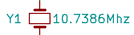
\includegraphics{icons/osci}     & Clock oscillator       \\
		\centering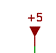
\includegraphics{icons/volt-5}   & 5 volts power supply   \\
		\centering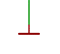
\includegraphics{icons/volt-gnd} & Ground power supply    \\
		\centering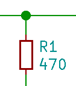
\includegraphics{icons/res}      & Resistor               \\
		\centering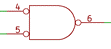
\includegraphics{icons/gate-and} & AND logic gate         \\
		\centering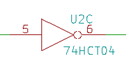
\includegraphics{icons/gate-inv} & Inverter logic gate    \\
	\end{tabular}
	\caption{Component symbols in schematic diagrams}
	\label{table:schematic-symbols}
\end{table}

If you still do not know what a bus, a capacitor or a logic gate is, do not panic. Most of these concepts will be elaborated in the following chapters.

\subsection{Schematic sheets}

TBD

\subsection{Multipart integrated circuits}

Some integrated circuits contain multiple parts under the same chip. Independent elements that operate separately but are encapsulated together. This is the case of most logic gates and many other logic functions such as encoders, decoders, multiplexers, etc. For example, the well known 7404 chip contains six logic inverters, each one using one input pin and one output pin. That is why it is known as an hex logic inverter. The same happens to the 7432, the quad 2-input OR gate that contains four independent functions. 

For legibility reasons, it is common to represent these multipart ICs in the schematic diagrams by separating each independent function as if it was a totally independent component. For example, the 7404 logic inverter is not represented as a single schematic component with six input pins and six output pins, but six separated logic gates with one single input and one single output. The main reason to do that is the each independent function is typically used in different parts of the design. For example, one of the inverters of a 7404 chip can be used in the CPU sheet while some other inverter of the same chip is used in the PSG circuit. This simplifies the reading, allowing you to focus on logic functions instead of chip pinout and connectivity. 

When multipart ICs are used in the schematic diagrams, the power pins of the IC {\tt VCC} and {\tt GND} are only represented in the first part of the IC. The reason is that most of the times we will want to add decoupling capacitors to the power pins. If you do not know yet what a coupling capacitor is, do not worry. We will discuss about this later. Just take the idea that power pins will be represented in the first part of the IC.

The figure \ref{fig:schematic-multipart-ics} shows an example of both things. There, the U9 chip is a 74HCU04 hex logic inverter. Here we can see three logic functions: {\tt U9A}, {\tt U9B} and {\tt U9C}. As you can see, the prefix {\tt U9} in all them indicate they belong to the same package, using letter suffixes to differentiate each function. Also, you can see how the power pins are only visible in {\tt U9A} but not in {\tt U9B}. That is because both parts share the same power inputs. The rest of the parts, {\tt U9D}, {\tt U9E} and {\tt U9F} are used in other schematic sheets, and they also do not show the power pins.

\begin{figure}[h]
	\centering
	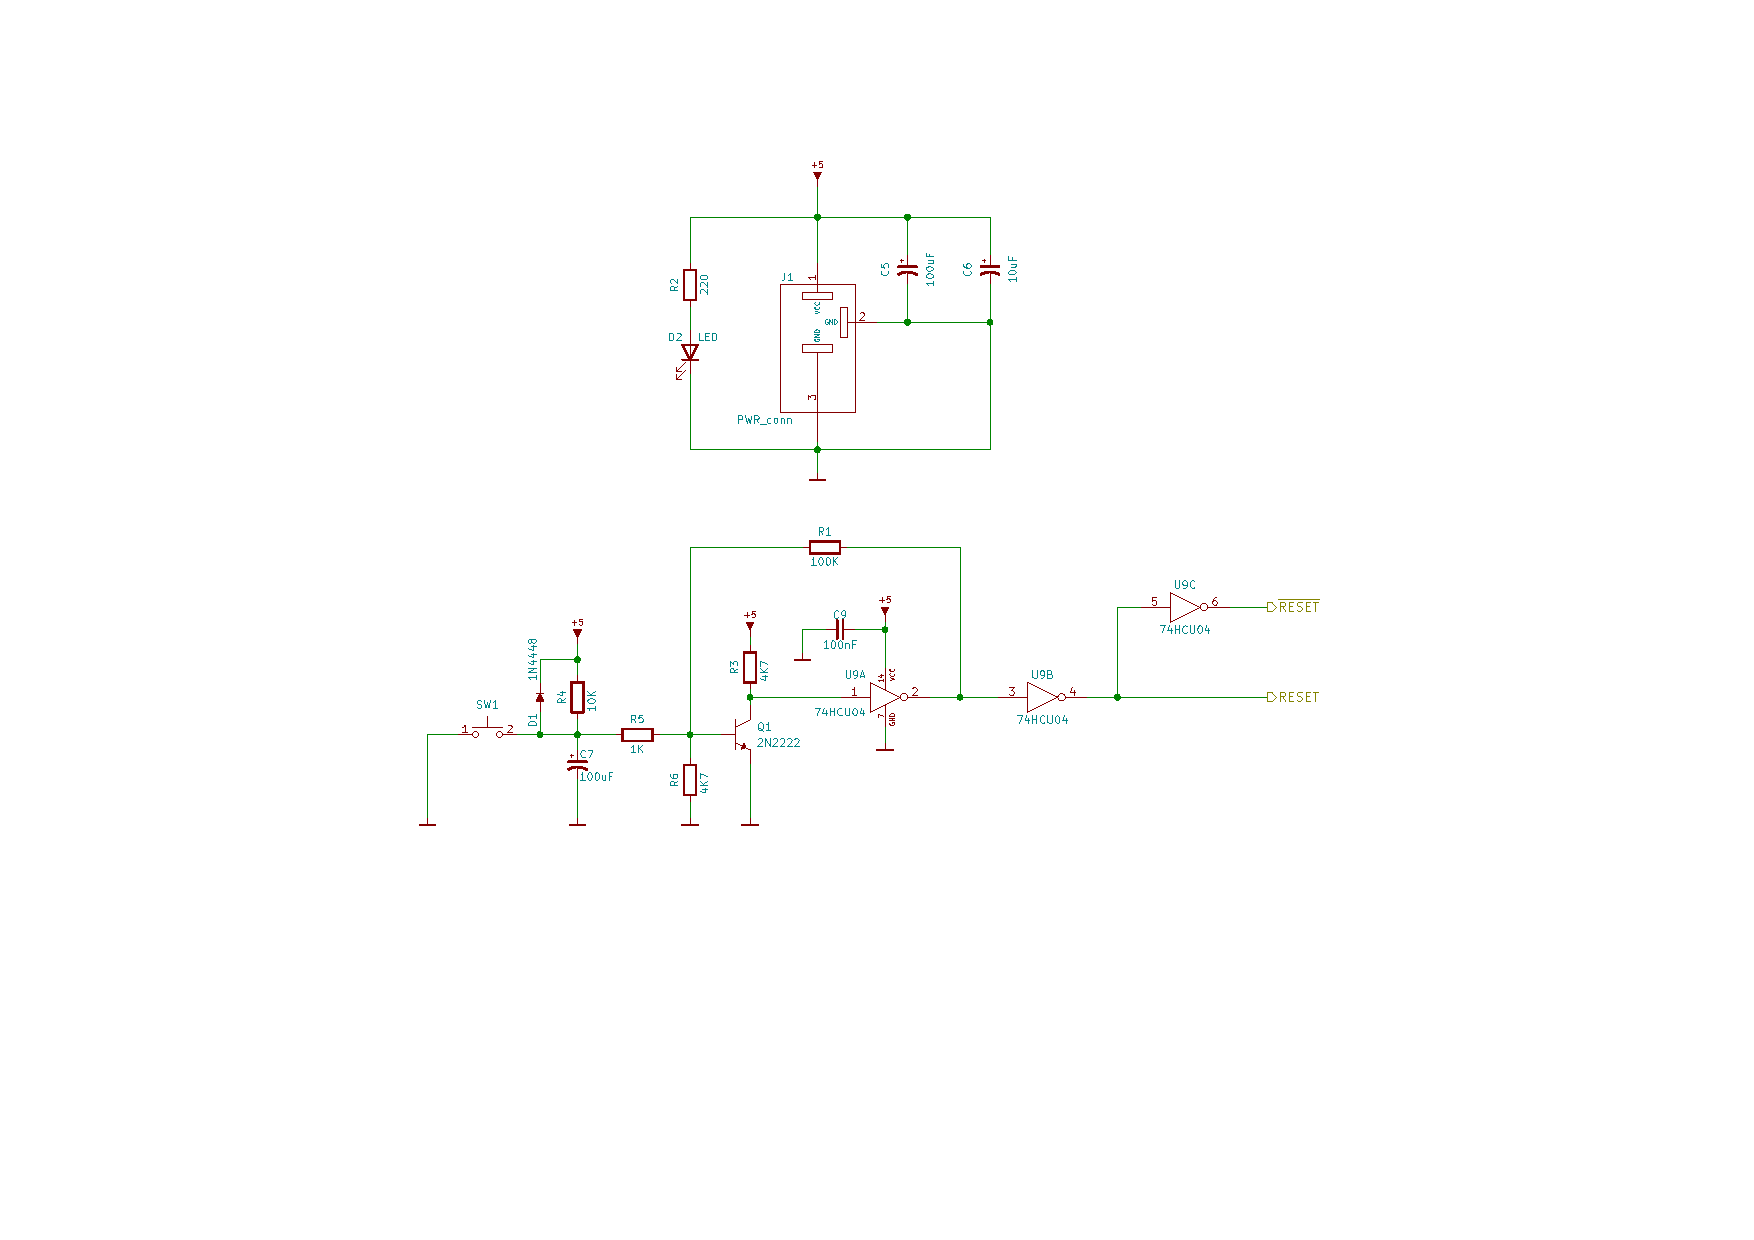
\includegraphics[width=0.7\linewidth,trim={12cm 7cm 8.5cm 8.5cm},clip]{figures/artemisa-schematic-power}
	\caption{Example of a multipart integrated circuit ({\tt U9}) in the schematic diagrams}
	\label{fig:schematic-multipart-ics}
\end{figure}


\subsection{Number notations}

Some numerical values are expressed along this manual. The prefix formats shown in Table \ref{table:number-formats} are used to distinguish between different integer bases. 

\begin{table}[h!]
	\centering
	\begin{tabular}{ r|l }
		{\bf Prefix} & {\bf Description}                               \\
		0b           & Binary number format. Example: 0b01100011.      \\
		0x           & Hexadecimal number format. Example: 0x4A0129FE. \\
	\end{tabular}
	\caption{Number format prefixes}
	\label{table:number-formats}
\end{table}
